\documentclass[11pt]{article}

% Related to page geometry
\usepackage[a4paper,vmargin={2.4cm,2.4cm},hmargin={2.4cm,2.4cm}]{geometry}
\usepackage[utf8]{inputenc}
\usepackage{amsmath}
\usepackage{caption}
\usepackage{graphicx}
\usepackage{float}

\author{Lucien Le Gall, Noé Casteleyn, Loris Manganelli}
\title{\textbf{Cooperative optimization - Numerical project :} Cooperative Kernel regression}
\date{March 31, 2026}

\begin{document}

\maketitle
The GitHub repository of our project (in particular the notebook) can be found at:
\begin{center}
\url{https://github.com/Loris-Manganelli/projet-cooperative-optimisation/tree/main}
\end{center}
\section{Part I : Data visualization and first 4 algorithms}
\subsection{Data visualization}
\begin{figure}[H]
    \centering
    \includegraphics[width=0.7\textwidth]{Figures/data_points_first_database.pdf}
    \caption{Visualization of the first database for the first 100 data points}
    \label{fig:first_database}
\end{figure}
\begin{figure}[H]
    \centering
    \includegraphics[width=0.7\textwidth]{Figures/data_points_second_database.pdf}
    \caption{Visualization of the second database for the first 100 data points}
    \label{fig:first_database}
\end{figure}
\subsection{Decentralized gradient descent and gradient tracking}
\subsubsection{Justification of the chosen step size}
Let us denote the agent $A_1, A_2, \dots, A_5$ (it also denotes the data points of the dataset belonging to this agent).
The function $f_i$ for each agent is:
\begin{equation}
    f_i(\alpha)=\dfrac{\sigma^2}{5}\dfrac{1}{2}\alpha^T K_{mm}\alpha+\dfrac{1}{2}\sum_{j\in A_i}(y_j-K_{(j)m}\alpha)^2+\dfrac{\nu}{10}\lVert \alpha \rVert^2
\end{equation}
One has:
\begin{equation}
    \nabla_{\alpha}f_i(\alpha)=\dfrac{\sigma^2}{5}K_{mm}\alpha-\sum_{j\in A_i}K_{(j)m}^T(y_i-K_{(i)m}\alpha) +\dfrac{\nu}{5}\alpha
    \label{eqn:grad}
\end{equation}
Then:
\begin{equation}
\nabla_{\alpha}^2f_i(\alpha)=\dfrac{\sigma^2}{5}K_{mm} + \sum_{j\in A_i} K_{(j)m}^T K_{(j)m}+\dfrac{\nu}{5}I_m
\end{equation}
So, let $\lambda_{i, \text{max}} = \underset{\lambda \in \mathrm{Sp}\big(\nabla_{\alpha}^2 f_i(\alpha)\big)}{\arg\max} |\lambda|$ for each agent $i$. Let $L=\max_i{|\lambda_{i, \text{max}}}|$. Then, we need to choose a step size which fulfilled is $\leq O\left(\dfrac{1}{L}\right)$. We have computed it using Python, and found $\dfrac{1}{L}\approx 0.010$. That is to say in the following $s\leq 10^{-2}$

\subsubsection{Convergence plots depending on graph structure}
\begin{figure}[H]
    \centering
    \includegraphics[width=0.7\textwidth]{Figures/DGD_GT_Fully_connected.pdf}
    \caption{Convergence of DGD and Gradient Tracking, in terms of $\lVert \alpha_i-\alpha^*\rVert$, on the Kernel ridge regression for a fully connected graph.}
\end{figure}

\begin{figure}[H]
    \centering
    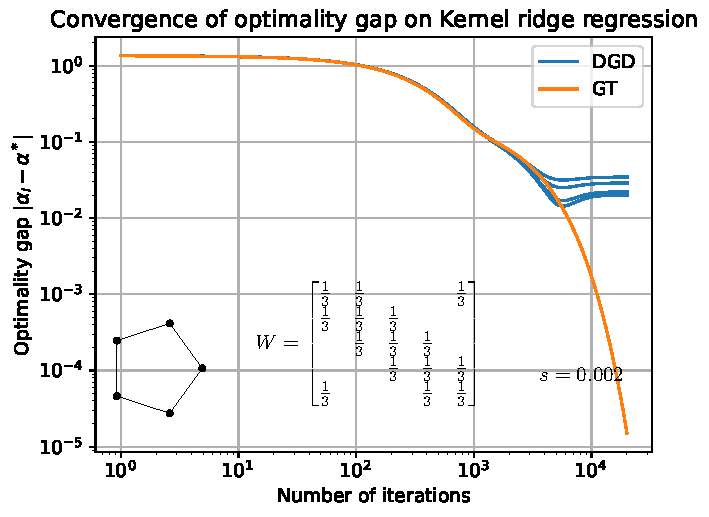
\includegraphics[width=0.7\textwidth]{Figures/DGD_GT_small_world.pdf}
    \caption{Convergence of DGD and Gradient Tracking, in terms of $\lVert \alpha_i-\alpha^*\rVert$, on the Kernel ridge regression for a circular graph.}
\end{figure}

\begin{figure}[H]
    \centering
    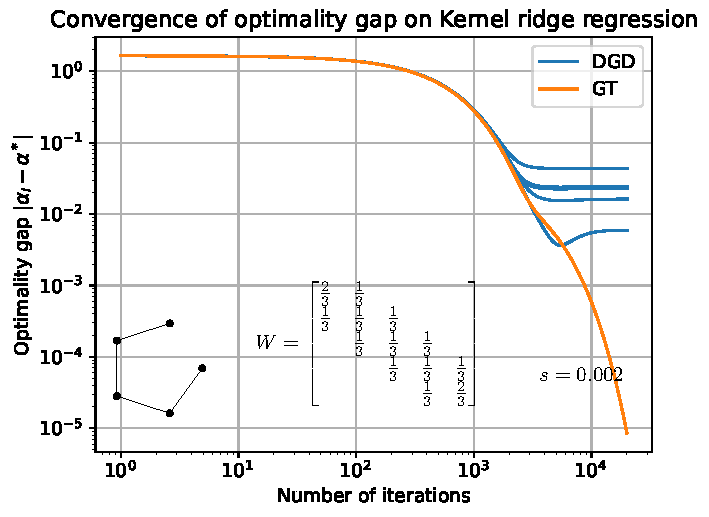
\includegraphics[width=0.7\textwidth]{Figures/DGD_GT_line.pdf}
    \caption{Convergence of DGD and Gradient Tracking, in terms of $\lVert \alpha_i-\alpha^*\rVert$, on the Kernel ridge regression for a line graph.}
\end{figure}

\textbf{Comments.} Concerning the DGD, we observe that the smaller the error ball, the better is the consensus. 
Indeed, one has theoretically that the error ball for DGD is $O\left(\dfrac{\alpha}{1-\gamma}\right)$ where $\dfrac{1}{1-\gamma}$ is the spectral gap of the graph, and $\alpha$ is the step size. We could reach zero error but slower, with a diminishing step size.
We also have an error on the consensus, which is of order $O\left(\dfrac{\alpha}{1-\gamma}\right)$.
The gradient tracking algorithm reaches zero error ball and zero consensus error.

\subsubsection{Visualization of the obtained function}
\begin{figure}[H]
    \centering
    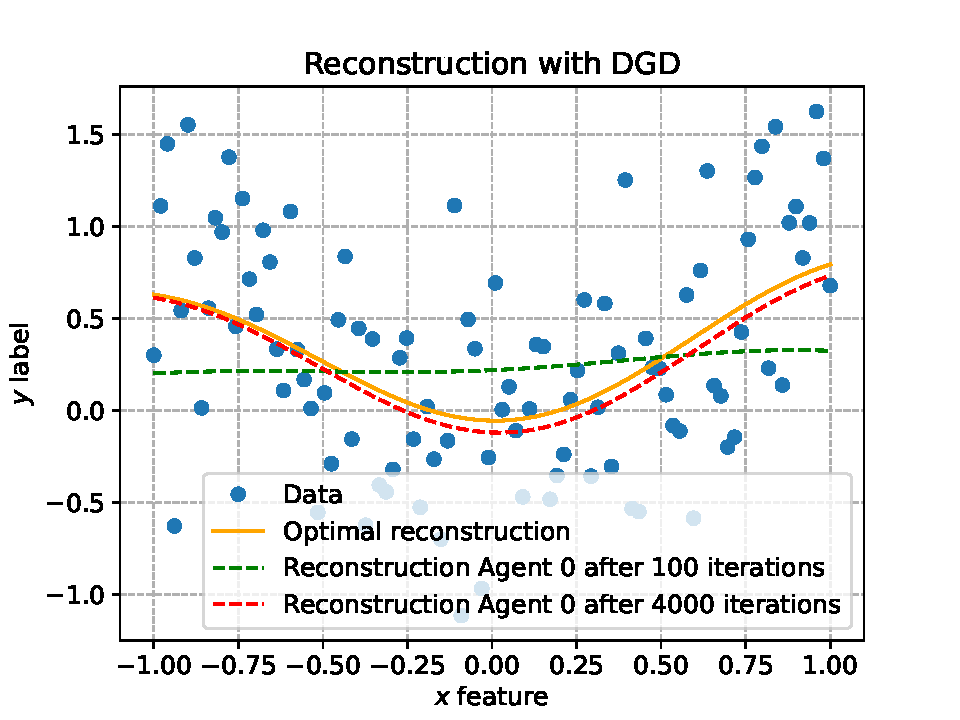
\includegraphics[width=0.7\textwidth]{Figures/RECONSTRUCTION_COMPARISON_DGD.pdf}
    \caption{Obtained function with DGD, for different number of iterations and comparison with the optimum}
\end{figure}
\begin{figure}[H]
    \centering
    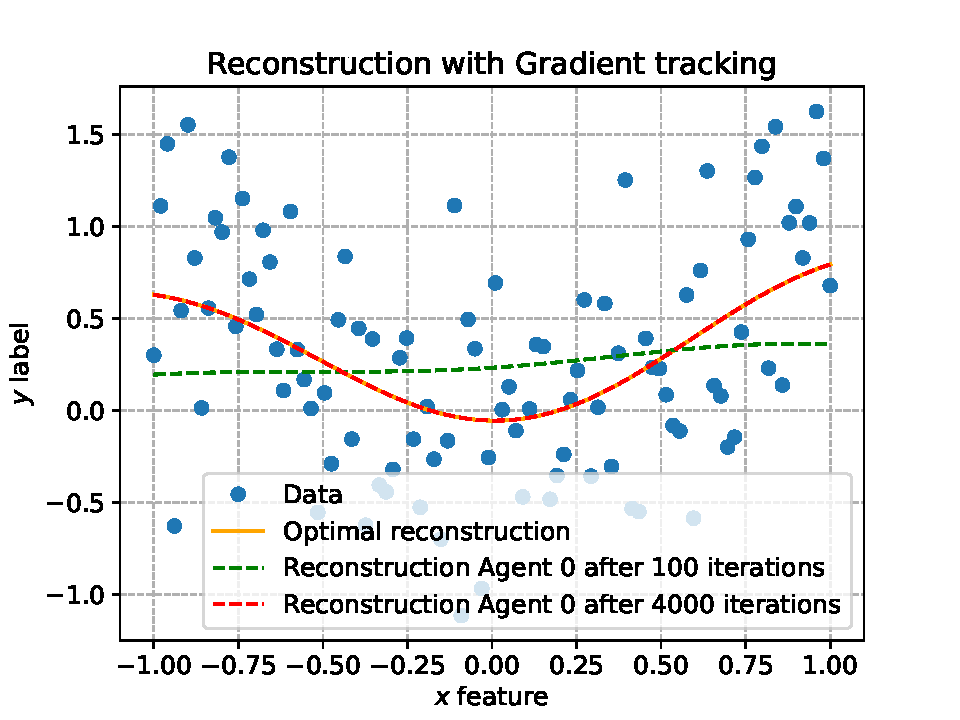
\includegraphics[width=0.7\textwidth]{Figures/RECONSTRUCTION_COMPARISON_GT.pdf}
    \caption{Obtained function with Gradient Tracking, for different number of iterations and comparison with the optimum}
\end{figure}

\textbf{Comments.} We clearly notice that the reconstruction after 100 iterations for the first agent is better for the gradient tracking method than for DGD. Moreover, after 4000 iterations, the reconstruction is quite satisfying for both methods meaning that we get really close to the optimum. The results are even better for ADMM and dual decomposition in terms of reconstruction (\textit{cf} notebook).

\subsection{Dual Methods (Dual decomposition and ADMM)}

We denote $F$ the following function:

\[F(y)=\sum_{i=1} f_i(x^i) \quad s.t. \quad Ay=0\]
Where $y =(x^i)_{1 \leq i\leq 5}$, And $A=I \otimes Id_m$, with $I$ the incidence matrix of the graph, where each edge is arbitrarily oriented.

\subsubsection{Justification of the stepzise}

The dual problem is $\sigma_{max}^2(I)/m$ -Smooth. Where $m=\max (m_i)$ is the strong convexity constant of $F$. In our case we find : $\texttt{step\_size}= O(10^{-2})$ typically $\texttt{step\_size} = 0.01$ is chosen.  

\subsubsection{Convergence plots}

\paragraph{Dual decomposition}

\begin{figure}[H]
    \centering
    \includegraphics[width=0.7\textwidth]{Figures/Dual Dec vs GT_line.pdf}
    \caption{Convergence of Dual Decomposition and Gradient tracking, in terms of $\lVert \alpha_i-\alpha^*\rVert$ on the Kernel ridge regression for a line  graph. The step size $s$ is for the dual decomposition only, $I$ is the oriented incidence matrix.}
\end{figure}

\begin{figure}[H]
    \centering
    \includegraphics[width=0.7\textwidth]{Figures/Dual Dec vs GT_small_world.pdf}
    \caption{Convergence of Dual Decomposition and Gradient tracking, in terms of $\lVert \alpha_i-\alpha^*\rVert$ on the Kernel ridge regression for a circular  graph. The step size $s$ is for the dual decomposition only, $I$ is the oriented incidence matrix.}
    
\end{figure}
\begin{figure}[H]
    \centering
    \includegraphics[width=0.7\textwidth]{Figures/Dual Dec vs GT_full.pdf}
    \caption{Convergence of Dual Decomposition and Gradient tracking, in terms of $\lVert \alpha_i-\alpha^*\rVert$ on the Kernel ridge regression for a full graph. The step size $s$ is for the dual decomposition only, $I$ is the oriented incidence matrix.}
\end{figure}

In the first two examples, a step size of $s=0.11$ is chosen, at the limit $2m/\sigma_{max}^2(I)$. However, for the fully connected graph, $\sigma_{max}^2(I)$ is twice bigger, so the algorithm doesn't converge anymore. 

When the graph is more connected, each solution converges faster to a consensus. 

\paragraph{ADMM} For ADMM the main parameter to play with is the $\beta$ parameter of the augmented Lagrangian.

\begin{figure}[H]
    \centering
    
\includegraphics[width=0.7\textwidth]{Figures/Comparison of Dual Dec, GT and ADMM.pdf}
    \caption{Convergence of ADMM ($\beta=1$), Dual Decomposition (step size $= 0.07$), and Gradient tracking (stepsize$= 0.02$), in terms of $\lVert \alpha_i-\alpha^*\rVert$ on the Kernel ridge regression.}
\end{figure}

We see that ADMM is faster than Dual decomposition and Gradient Tracking with  step sizes chosen optimally. We chose $\beta=1$ because of the next result: 
\begin{figure}[H]
    \centering
    
\includegraphics[width=0.7\textwidth]{Figures/Comparison of Different Beta Values.pdf}
    \caption{Convergence of ADMM ($\beta=1$) for different $\beta$ constant, and Dual Decomposition (step size $= 0.07$), in terms of $\lVert \alpha_i-\alpha^*\rVert$ on the Kernel ridge regression for a full  graph.}
\end{figure}

\subsection{Increasing $n$}
Our results on the different methods when increasing $n$, while using $m\approx\sqrt{n}$, are the following one (we used adaptive step size to counter effect the diminishing smoothness constant).

\begin{figure}[H]
    \centering
    \includegraphics[scale=0.5]{Figures/final_gaps.pdf}
    \caption{Final gap when increasing $n$ for the different methods}
    \label{fig:my_label}
\end{figure}

We measure the gap as the average over agent of final optimally gap.
We notice that the gradient in the term \ref{eqn:grad} is higher (because we sum more terms), so the term $\dfrac{1}{L}$ decreases resulting in slower convergence. 

\section{Part II}

\begin{figure}[H]
    \centering
    
\includegraphics[width=0.7\textwidth]{Figures/FedAVG_B20_C5_E.pdf}
    \caption{Convergence of FedAVG in terms of $\lVert F(\alpha_i)-F(\alpha^*)\rVert$ on the Kernel Ridge Regression example, for a constant learning rate of 0.002, and varying the number of epochs $E$}
    \label{fig:FedAVG_E}
\end{figure}

\begin{figure}[H]
    \centering
    
\includegraphics[width=0.7\textwidth]{Figures/FedAVG_E5_C5_B.pdf}
    \caption{Convergence of FedAVG in terms of $\lVert F(\alpha_i)-F(\alpha^*)\rVert$ on the Kernel Ridge Regression example, for a constant learning rate of 0.002, and varying the batch size $B$}
    \label{fig:FedAVG_B}
\end{figure}

\begin{figure}[H]
    \centering
    
\includegraphics[width=0.7\textwidth]{Figures/FedAVG_E5_B20_C.pdf}
    \caption{Convergence of FedAVG in terms of $\lVert F(\alpha_i)-F(\alpha^*)\rVert$ on the Kernel Ridge Regression example, for a constant learning rate of 0.002, and varying the number of devices $C$}
    \label{fig:FedAVG_C}
\end{figure}

\paragraph{Comments.} In the case $B=20$ (full-batch case) and $E=1$, we can observe that the FedAVG algorithm boils down to DGD. That is why, on figure \ref{fig:FedAVG_E}, we observe an error that goes to 0 asymptotically. Results observed on figures \ref{fig:FedAVG_B} are expected, since reducing the batch-size brings us closer to a stochastic gradient algorithm, which is known for stopping to improve sooner than the full-batch setting. Finally,, figure \ref{fig:FedAVG_C} is also pretty intuitive, since using less data obviously leads to less qualitative results. It is however surprising to note that using $C=2$ devices leads to better results than using $C=3$.

\section{Part III}
We notice that we obtained convergence for $\epsilon=10$, and $\epsilon=1$. For $\epsilon=10$, the performance is degraded, although the theoretical guarantees still hold.
\begin{figure}[H]
    \centering
    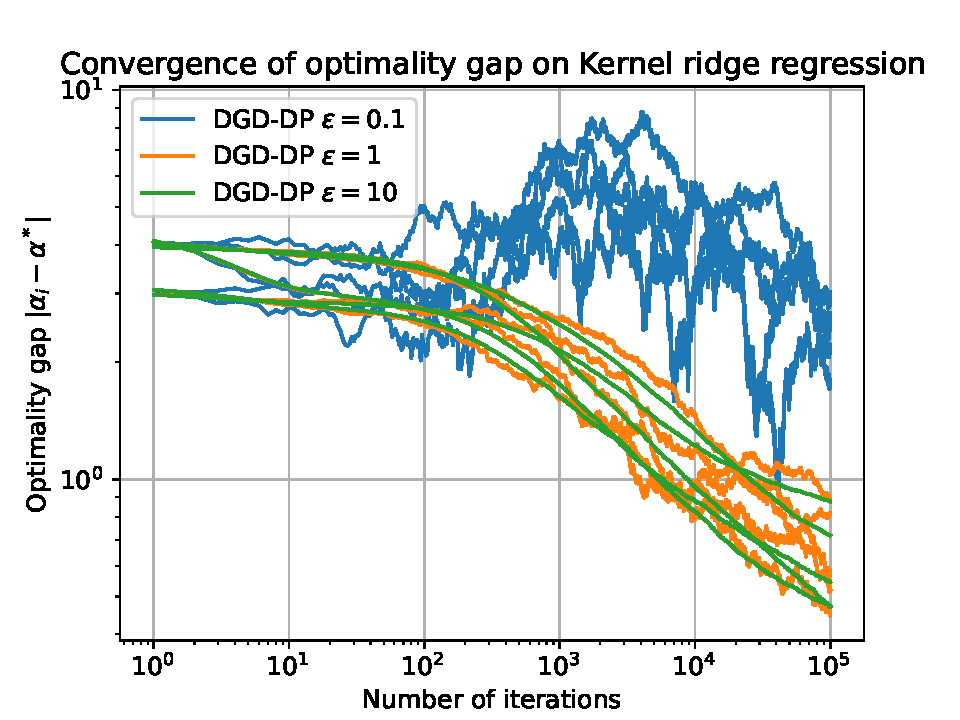
\includegraphics[width=0.62\textwidth]{Figures/GAP_DGD_DP.pdf}
    \caption{Convergence of DGD-DP in terms of $\lVert \alpha_i-\alpha^*\rVert$ for a line graph}
\end{figure}

\end{document}
